\documentclass[letterpaper,10pt,oneside]{article}

\usepackage[style=authoryear, backend=biber, natbib=true]{biblatex}

\bibliography{mybib}

\usepackage{graphicx}
\graphicspath{ {/Users/jacksonwills/Documents/Fitz_Research/Report} }

\usepackage{amsmath, amssymb, amsfonts, bm, mathtools}
\usepackage{hyperref}

\usepackage[autoload=true]{jlcode}



\title{System Modeling and Control of the Furuta Pendulum}
\author{Jackson Wills}



\begin{document}

\maketitle

\tableofcontents

\newpage

\section{System Decription}

In this paper, the dynamics of the Furuta Pendulum are simulated and the system is given reasonable parameters and controlled using linear full-state feedback control. The Furuta Pendulum was developed by a man named Katsuhisa Furuta at the Tokyo Institute of Technology in 1992. The device consists of an motor which can rotate a beam in the horizontal plane. Attatched to that beam is a pendulum which is free to rotate in the vertical plane - see figure \ref{fig:diagram}. The end goal of this project was to use my control law to control a real life Furuta Pendulum that Dr. Fitzgerald has in his lab.


\begin{figure}[!ht]
  % The [!ht] puts the figure right here instead of at the top of the page, which is the default. It gives me a warning "'!h' float specifier changed to '!ht'"
  \centering
  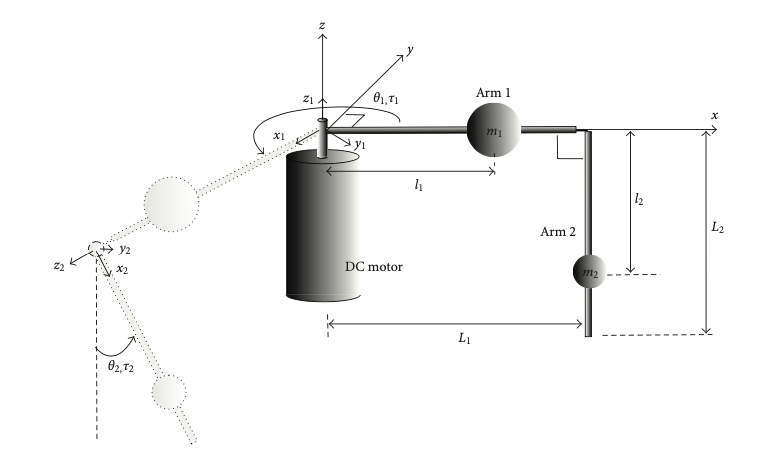
\includegraphics[width=0.9\textwidth]{FurutaDiagram}
  % This makes the diagram be .9 times the width of the text!
  \caption{A diagram of the Furuta Pendulum \citep{DYNAMICS}}
  \label{fig:diagram}
  % label is cool! This lets me refernce the figure, even when the figure number changes.
\end{figure}

\section{Derivation of the Equations of Motion}

The first thing to do is to get equations of motion which accurately model the system. These equations were derived largely with the help of \cite{DYNAMICS}. These equations were derived using a jupider notebook (The code is found in the appendix \ref{EOM}). To make these equations it was assumed that both rods are infitely stiff. All damping was assumed to be viscous. The equations of motion were found using Lagrange’s equation. First, two rotation matrices were found.

\begin{align}
  R1 &= \left[\begin{matrix}
  \cos{\left(\theta_{1}{\left(t \right)} \right)} & \sin{\left(\theta_{1}{\left(t \right)} \right)} & 0 \\
  - \sin{\left(\theta_{1}{\left(t \right)} \right)} & \cos{\left(\theta_{1}{\left(t \right)} \right)} & 0 \\
  0 & 0 & 1
  \end{matrix}\right] \\
  R2 &= \left[\begin{matrix}
  0 & \sin{\left(\theta_{2}{\left(t \right)} \right)} & - \cos{\left(\theta_{2}{\left(t \right)} \right)} \\
  0 & \cos{\left(\theta_{2}{\left(t \right)} \right)} & \sin{\left(\theta_{2}{\left(t \right)} \right)} \\
  1 & 0 & 0
  \end{matrix}\right]
\end{align}
Position vectors were found (each in its own reference frame)
\begin{align}
  r_{1} &=
  \left[\begin{matrix}
  l_{1} \\
  0 \\
  0
  \end{matrix}\right] \\
  r_{2} &=
  \left[\begin{matrix}
  l_{2} \\
  0 \\
  0
  \end{matrix}\right]
\end{align}


Next, the linear and rotational velocities were found. $v_{1}$ is the total linear velocity of arm 1 and $v_{2}$ is the total linear velocity of arm 1. Similarly, $\omega_{1}$ is the rotational velocity of arm 1 and $\omega_{2}$ is the rotational velocity of arm 1.

\begin{align}
  v_{1} &=
  \left[\begin{matrix}
  0 \\
  l_{1} \dot{\theta}_{1} \\
  0\end{matrix}\right] \\
  \omega_{1} &=
  \left[\begin{matrix}
  0 \\
  0 \\
  \dot{\theta}_{1}
  \end{matrix}\right] \\
  v_{2} &=
  \left[\begin{matrix}
  L_{1} \dot{\theta}_{1} \sin{\left(\theta_{2}{\left(t \right)} \right)} \\
  L_{1} \dot{\theta}_{1} \cos{\left(\theta_{2}{\left(t \right)} \right)} + l_{2} \dot{\theta}_{2} \\
  - l_{2} \dot{\theta}_{1} \sin{\left(\theta_{2}{\left(t \right)} \right)}
  \end{matrix}\right] \\
  \omega_{2} &=
  \left[\begin{matrix}
  - \dot{\theta}_{1} \cos{\left(\theta_{2}{\left(t \right)} \right)} \\
  \dot{\theta}_{1} \sin{\left(\theta_{2}{\left(t \right)} \right)} \\
  \dot{\theta}_{2}
  \end{matrix}\right]
\end{align}


The kinetic energies of each arm were added together and the same was done for the potential energies. The arms each have point masses $m_{1}$ and $m_{2}$ respectively. The inertial tensors of each arm are given by:

\begin{align}
  J_{1} &=
  \left[\begin{matrix}
  J_{1xx} & 0 & 0 \\
  0 & J_{1yy} & 0 \\
  0 & 0 & J_{1zz}
  \end{matrix}\right] \\
  J_{2} &=
  \left[\begin{matrix}
  J_{2xx} & 0 & 0 \\
  0 & J_{2yy} & 0 \\
  0 & 0 & J_{2zz}
  \end{matrix}\right]
\end{align}


The Lagrangian was created.

\begin{multline}
  L =
  0.5 J_{1zz} \dot{\theta}_{1}^{2} + 0.5 J_{2xx} \dot{\theta}_{1}^{2} \cos^{2}{\left(\theta_{2}{\left(t \right)} \right)}
   + 0.5 J_{2yy} \dot{\theta}_{1}^{2} \sin^{2}{\left(\theta_{2}{\left(t \right)} \right)}
      \\
    + 0.5 J_{2zz} \dot{\theta}_{2}^{2} + 0.5 L_{1}^{2} m_{2} \dot{\theta}_{1}^{2} \sin^{2}{\left(\theta_{2}{\left(t \right)} \right)}
   - g l_{2} m_{2} \left(1 - \cos{\left(\theta_{2}{\left(t \right)} \right)}\right) + 0.5 l_{1}^{2} m_{1} \dot{\theta}_{1}^{2}
      \\
    + 0.5 l_{2}^{2} m_{2} \dot{\theta}_{1}^{2} \sin^{2}{\left(\theta_{2}{\left(t \right)} \right)}
    + 0.5 m_{2} \left(L_{1} \dot{\theta}_{1} \cos{\left(\theta_{2}{\left(t \right)} \right)} + l_{2} \dot{\theta}_{2}\right)^{2}
\end{multline}

Using Lagrange's equations, the equations of motion were found to be \\

\begin{multline}
  0 = - 2.0 J_{2xx} \dot{\theta}_{1} \dot{\theta}_{2} \sin{\left(\theta_{2}{\left(t \right)} \right)} \cos{\left(\theta_{2}{\left(t \right)} \right)} + 2.0 J_{2yy} \dot{\theta}_{1} \dot{\theta}_{2} \sin{\left(\theta_{2}{\left(t \right)} \right)} \cos{\left(\theta_{2}{\left(t \right)} \right)}
        \\
   + 1.0 L_{1} l_{2} m_{2} \ddot{\theta}_{2} \cos{\left(\theta_{2}{\left(t \right)} \right)} - 1.0 L_{1} l_{2} m_{2} \dot{\theta}_{2}^{2} \sin{\left(\theta_{2}{\left(t \right)} \right)} + b_{1} \dot{\theta}_{1} + \\ 2.0 l_{2}^{2} m_{2} \dot{\theta}_{1} \dot{\theta}_{2} \sin{\left(\theta_{2}{\left(t \right)} \right)} \cos{\left(\theta_{2}{\left(t \right)} \right)} - \tau_{1}
    \\
    + \ddot{\theta}_{1} \left[1.0 J1zz + 1.0 J_{2xx} \cos^{2}{\left(\theta_{2}{\left(t \right)} \right)} + 1.0 J_{2yy} \sin^{2}{\left(\theta_{2}{\left(t \right)} \right)} + 1.0 L_{1}^{2} m_{2} \sin^{2}{\left(\theta_{2}{\left(t \right)} \right)}
      \right.
      \\
      \left.
     + 1.0 L_{1}^{2} m_{2} \cos^{2}{\left(\theta_{2}{\left(t \right)} \right)} + 1.0 l_{1}^{2} m_{1} + 1.0 l_{2}^{2} m_{2} \sin^{2}{\left(\theta_{2}{\left(t \right)} \right)}\right]
\end{multline}

      % It is important that the new line of the equation starts with an + or minus

      % I put these left. and right. in there bacause the parentesis went over a line break that I wanted to make.      Note the periods after the left. and right.        Also, I made the parentesis that crossed the line into a braket to make it clearer. I don't think this is necessary and it may even be bad practice.
      % Also, I guess it breaks if you comment inside the multline...?

% I used multline to create a math enviornment, but thats only because the equations were so long. align is better for shorter things. The & symbol is where the two equations align themselves. Shown here is an unrelated example of align.
%\begin{align}
  %x &= \left( 2 + \frac{1}{3} \right) %\label{eq:important}\\
  %y &= 4x
%\end{align}
% Some random text. See \eqref{eq:important} for blah.
\begin{multline}
  0 = 1.0 J_{2zz} \ddot{\theta}_{2} + 1.0 L_{1} l_{2} m_{2} \ddot{\theta}_{1} \cos{\left(\theta_{2}{\left(t \right)} \right)} + b_{2} \dot{\theta}_{2} + g l_{2} m_{2} \sin{\left(\theta_{2}{\left(t \right)} \right)}
      \\
   + 1.0 l_{2}^{2} m_{2} \ddot{\theta}_{2} - \tau_{2} + \dot{\theta}_{1}^{2} \left[1.0 J_{2xx} \sin{\left(\theta_{2}{\left(t \right)} \right)} \cos{\left(\theta_{2}{\left(t \right)} \right)}
\right.
\\
\left.
   - 1.0 J_{2yy} \sin{\left(\theta_{2}{\left(t \right)} \right)} \cos{\left(\theta_{2}{\left(t \right)} \right)} - 1.0 l_{2}^{2} m_{2} \sin{\left(\theta_{2}{\left(t \right)} \right)} \cos{\left(\theta_{2}{\left(t \right)} \right)}\right]
\end{multline}

\section{Linearization}

These equations of motion were then linearized about $\theta_{1}=0$ and $\theta_{2}=\pi$ \\
The code that did this can be found in the appendix under \ref{Code:Linearization}. Variables were changed according to the following rules:
\begin{align}
 \tau_{1} => u_{1}, \\  \tau_{2} => u_{2}, \\  \theta_{1}{\left(t \right)} => z_{1}, \\  \theta_{2}{\left(t \right)} => z_{2}, \\  \frac{d}{d t} \theta_{1}{\left(t \right)} => z_{3}, \\  \frac{d}{d t} \theta_{2}{\left(t \right)} => z_{4} \\
\end{align}

Cordinates were shifted by $z = x - x_{0}$ and $r = u - u_{0}$. The resulting linear equations are:

\begin{multline}
\left[\begin{matrix}
  \dot{z}_{1} \\
  \dot{z}_{2} \\
  \dot{z}_{3} \\
  \dot{z}_{4}
\end{matrix}\right]
=
  \left[\begin{matrix}
  0 & 0 & 1 & 0 \\
  0 & 0 & 0 & 1 \\
  0 & \frac{1.0 L_{1} g l_{2}^{2} m_{2}^{2}}{\hat{J}_{0} \hat{J}_{2} - L_{1}^{2} l_{2}^{2} m_{2}^{2}} & \frac{\hat{J}_{2} b_{1}}{- \hat{J}_{0} \hat{J}_{2} + L_{1}^{2} l_{2}^{2} m_{2}^{2}} & \frac{1.0 L_{1} b_{2} l_{2} m_{2}}{- \hat{J}_{0} \hat{J}_{2} + L_{1}^{2} l_{2}^{2} m_{2}^{2}} \\
  0 & \frac{1.0 \hat{J}_{0} g l_{2} m_{2}}{\hat{J}_{0} \hat{J}_{2} - L_{1}^{2} l_{2}^{2} m_{2}^{2}} & \frac{L_{1} b_{1} l_{2} m_{2}}{- \hat{J}_{0} \hat{J}_{2} + L_{1}^{2} l_{2}^{2} m_{2}^{2}} & \frac{1.0 \hat{J}_{0} b_{2}}{- \hat{J}_{0} \hat{J}_{2} + L_{1}^{2} l_{2}^{2} m_{2}^{2}}
  \end{matrix}\right]
  \left[\begin{matrix}
    z_{1} \\
    z_{2} \\
    z_{3} \\
    z_{4}
  \end{matrix}\right]
  \\
  +
  \left[\begin{matrix}
  0 & 0 \\
  0 & 0 \\
  \frac{\hat{J}_{2}}{- \hat{J}_{0} \hat{J}_{2} + L_{1}^{2} l_{2}^{2} m_{2}^{2}} & \frac{1.0 L_{1} l_{2} m_{2}}{\hat{J}_{0} \hat{J}_{2} - L_{1}^{2} l_{2}^{2} m_{2}^{2}} \\
  \frac{L_{1} l_{2} m_{2}}{\hat{J}_{0} \hat{J}_{2} - L_{1}^{2} l_{2}^{2} m_{2}^{2}} & \frac{1.0 \hat{J}_{0}}{- \hat{J}_{0} \hat{J}_{2} + L_{1}^{2} l_{2}^{2} m_{2}^{2}}
  \end{matrix}\right]
  \left[\begin{matrix}
    r_{1} \\
    r_{2}
  \end{matrix}\right]
\end{multline}


\section{The Control Law}

The goal of the control law was to keep $\theta_{2}=\pi$, assuming the system starts near $\pi$. \\

A linear full-state feedback control law was implemented. The slowest two poles were placed with an overshoot of 5 percent and a settle time of 0.3 seconds. The faster poles were placed at a settle time five times faster than the slow poles, but at the same $\zeta$ value. The resulting gain matrix was found using Ackermann's formula \ref{Control_Modeling}: \\

% one way to do it
    %$ k =
      %\begin{bmatrix}
        %8.53 &
          %-15.90 &
            %-3.66 &
              %-0.97
                %\end{bmatrix}$

\begin{align}
  k = \left[\begin{array}{cccc}
  8.53 &
  -15.90 &
  -3.66 &
  -0.97
  \end{array}\right]
\end{align}
It should be noted that I assumed full knowledge of all states. In real life, we would have measured $\theta_{1}$ and $\theta_{2}$ and taken whatever 'dirty derivatives' are to find $\dot{\theta}_{1}$ $\dot{\theta}_{2}$.
\section{Conclusion}
The system was modeled in Julia, but there is not way that I am aware of a way to put any sort of animation inside a PDF. So here is a still image of the the animation in figure \ref{Animation}.
\clearpage
\begin{figure}[!h]
  \centering
  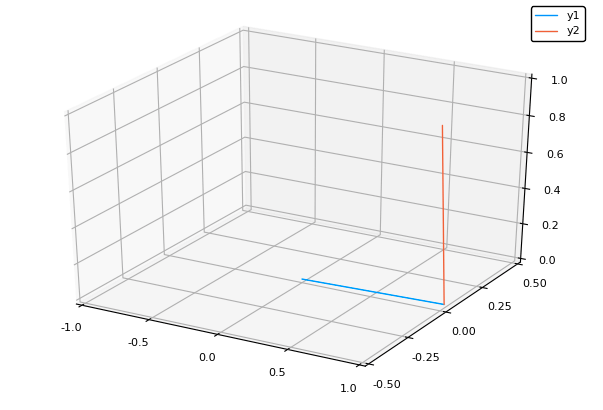
\includegraphics[width=1.0\textwidth]{AnimationPic}
  \caption{My Modeling of the Furuta Pendulum}
  \label{Animation}
\end{figure}


And there you have it! The magical two lines that don't move that all of this was about!
I was also supposed to try to make a swing up controller, and I'd like to give a shout out to \cite{SWINGUP} for trying to help me with that, but it was just really hard....


\clearpage

\appendix
\section{Code Files}

\subsection{EOM Derivation}
\label{EOM}
\begin{figure}[!h]
  % The [!h] puts the figure right here instead of at the top of the page, which is the default.
  \centering
  \includegraphics[width=1.0\textwidth]{Furuta_Pendulum_EOM_page1}
\end{figure}

\begin{figure}[!h]
  \centering
  \includegraphics[width=1.0\textwidth]{Furuta_Pendulum_EOM_page2}
\end{figure}
\clearpage

\subsection{Linearization}
\label{Code:Linearization}
\begin{figure}[!h]
  % The [!h] puts the figure right here instead of at the top of the page, which is the default.
  \centering
  \includegraphics[width=1.0\textwidth]{My_Furuata_Lineraization_page1}
\end{figure}

\begin{figure}[!h]
  % The [!h] puts the figure right here instead of at the top of the page, which is the default.
  \centering
  \includegraphics[width=1.0\textwidth]{My_Furuata_Lineraization_page2}
\end{figure}

\begin{figure}[!h]
  % The [!h] puts the figure right here instead of at the top of the page, which is the default.
  \centering
  \includegraphics[width=1.0\textwidth]{My_Furuata_Lineraization_page3}
\end{figure}

\begin{figure}[!h]
  % The [!h] puts the figure right here instead of at the top of the page, which is the default.
  \centering
  \includegraphics[width=1.0\textwidth]{My_Furuata_Lineraization_page4}
\end{figure}

\clearpage
\subsection{Control and Modeling}
\label{Control_Modeling}
\lstinputlisting{Furuta_Control_Modeling.jl}
%I was able to put julia code in here because of the jlcode.sty that is in this Report Folder.



\clearpage
%use clearpage instead of newpage because some objects dont care about new pages (these are called floats, and the bibliography is one of them) but they do care about clearpages!

\printbibliography

\end{document}
